\section{SOLID principer} \label{chap:solid}
Nogle SOLID principper er blevet benyttet og vil herunder blive gennemgået med kodeeksempler.

\subsection{Single responsibility principle} \label{sec:solid_s}
I forbindelse med at designe programmet efter mønstre som nævnt i forrige kapitel, har det også været naturligt at opdele klasser til kun af have et enkelt formål. Det ses som eksempel på \textit{Persistency} klasserne \texttt{ProjectRepository.java} og \texttt{EmployeeRepository}, der henholdsvis har ansvaret for at håndtere de primære hovedobjekt-klasser; \textit{Employee's} og \textit{Project}'s.

Derudover er alle klassers metoder som udgangspunkt lavet til at kun at have et enkelt formål. Herunder i \ref{lst:single_responsibility_source} er to eksempler på metoder fra \texttt{Employee.java}, hvis eneste formål er at validere det givne argument.
\begin{listing}[H]
    \centering
    \caption{Single responsibility metoder}\label{lst:single_responsibility_source}
    \begin{minted}[breaklines]{java}
  private String validateFirstName(String firstName) throws InvalidPropertyException {
    if (firstName.length() < 2) {
      throw new InvalidPropertyException("Fornavn mangler");
    }
    return firstName;
  }

  private String validateLastName(String lastName) throws InvalidPropertyException {
    if (lastName.length() < 2) {
      throw new InvalidPropertyException("Efternavn mangler");
    }
    return lastName;
  }

    \end{minted}
\end{listing}
Der er dog enkelte metoder, der kunne optimeres i forhold til \textit{Single resposibility} principet. Her kan nævnes \textit{createProjectActivity()} som beskrevet i \textit{White box test} \ref{chap:white_box_create_project_activity} kapitlet. Denne metode er både ansvarlig for at acceptere om en medarbejder kan oprette en projekt aktiviet, og derefter også at oprette den. Her kunne man refaktorere til, at tjekket om medarbejderen må oprette en aktivitet, lå udenfor metoden.

\subsection{Open/closed principle} \label{sec:solid_o}
Det lyder fra opgaveformuleringen, at der skal være mulighed for at opdele projekter op i aktiviteter, og at der skal være mulighed for at lave faste aktiviteter til registrering af bl.a. ferie og kurser, som ikke er knyttet til projekter. Et simpelt eksempel hvor \textit{Open/Closed}-princippet er blevet benyttet til at imødekomme førnævnte er at lave en abstrakt klasse kaldet \texttt{activity}, som vist herunder i figur \ref{fig:class_activity_example}.

\begin{figure}[H]
    \centering
    \caption{Klassediagram af \textit{aktivity} klasserne}
    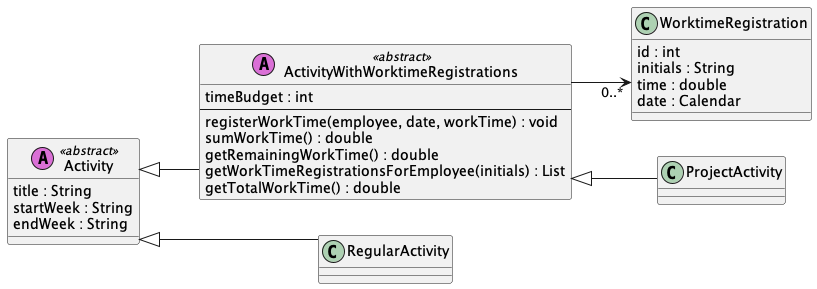
\includegraphics[width = 12cm, keepaspectratio]{TaskFusion/out/assets/diagrams/class_liskov_model_example/liskov_model_example.png}
    \label{fig:class_activity_example}
\end{figure}
Vi skelner i programmet imellem en fast aktivitet og en projekt aktivitet, hendholdsvis \texttt{RegularActivity} og \texttt{ProjecActivity}. Begge typer har behov for egenskaberne \textit{title}, \textit{startWeek} og \textit{endWeek}. For at sikre at kunne overholde de forventninger der er til disse egenskaber, er disse i en abstrakt klasse \texttt{Activity}, som underklasserne nedarver fra. På den måde er \texttt{Activity} lukket for ændringer men åben for udvidelser. 

Der er desuden også det argument, at \textit{single responsibilty princippet} bliver fulgt, da \texttt{Activity} klassen kun har én grund til at blive ændret. Den grund vil indbefatte en ændring af definitionen, af hvad en aktivitet er, f.eks. en ændring af dets felter.

\subsection{Liskov substitution principle} \label{sec:solid_l}
Derudover skal projekt aktiviteter kunne håndtere tidsregistreringer. Istedet for at fylde \texttt{ProjectActivity}-klassen med metoder, nedarves igen fra en abstrakt klasse \texttt{ActivityWithWorktimeRegistration}, se igen klassediagram \ref{fig:class_activity_example}. På denne måde kan metoder relateret til tidsregistrering ikke kaldes fra \texttt{RegularActivity}, og det er samtidig muligt at udvide senere med aktiviteter der kan have tidsregisteringer eller ej.

\subsection{Interface segregation principle} \label{sec:solid_i}
Facade-laget bruges som mellemlag mellem præsentations- og program-lag, og på den måde afkobler forskellige dele af programmet. Ser vi nærmere på facade-laget, har vi også her forsøgt at reducere sammenkoblingen mellem høj- og lavniveaus komponenter, ved at afhænge af abstraktioner istedet for konkrete implementeringer. Det er gjort ved brug af \textit{interfaces} der afkobler \texttt{TaskFusion} fra henholdsvis \texttt{EmployeeFacade} og \texttt{ProjectFacade}, som vist herunder i figur \ref{fig:class_facade_full}. Et udvidet klassediagram over facade-laget kan ses i appendix \ref{apdx:classDiagram_facade_full}.

\begin{figure}[H]
    \centering
    \caption{Klassediagram af facade-laget}
    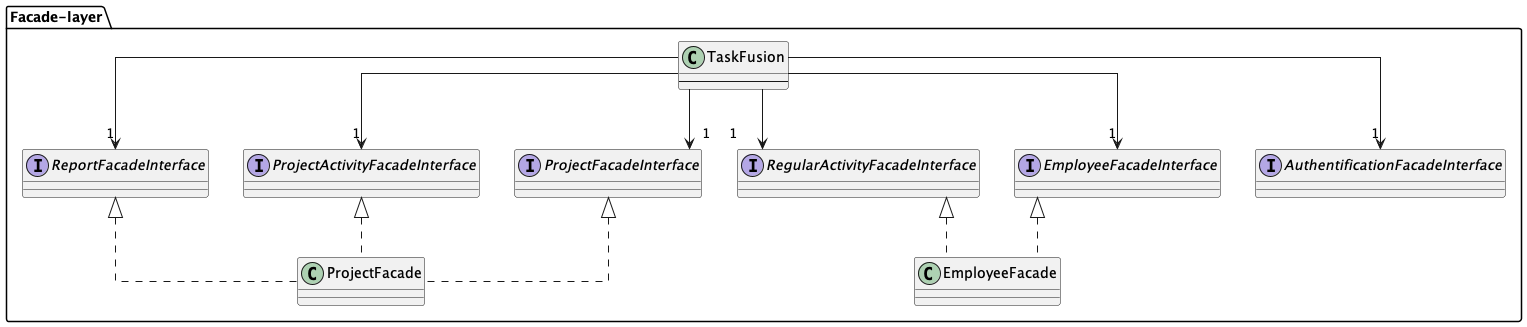
\includegraphics[width = \textwidth, keepaspectratio]{TaskFusion/out/assets/diagrams/class_facade_layer_simple/ClassDiagram_facade_simple.png}
    \label{fig:class_facade_simple}
\end{figure}

Ser vi istedet på koblingen mellem \textit{facade}- og \textit{persistency}-laget, kan vi her forbedre programmet i forhold til \textit{Interface segragation principle}. Den nuværende implementation ser ud som vist herunder i figur \ref{fig:class_facade_persistency_current}

\begin{figure}[H]
    \centering
    \caption{Klassediagram af nuværende forbindelse mellem facade- og persistency-laget}
    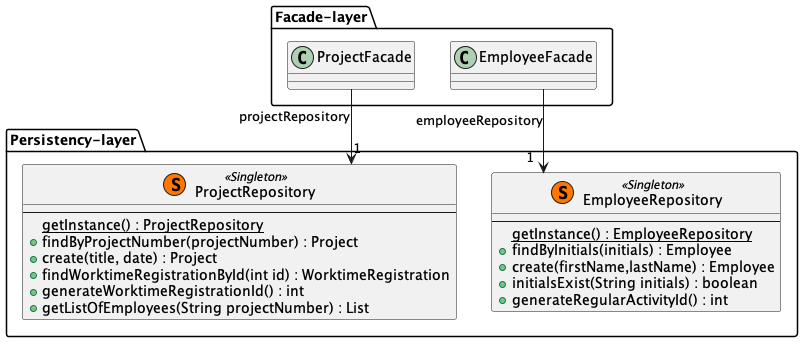
\includegraphics[width = 12cm, keepaspectratio]{TaskFusion/out/assets/diagrams/class_persistency_to_facade/persistency_to_facade_example.png}
    \label{fig:class_facade_persistency_current}
\end{figure}

Som programmet er nu, afhænger \texttt{EmployeeFacade} og \texttt{ProjectFacade} direkte af implemterede metoder i henholdsvis \texttt{EmployeeRepository} og \texttt{ProjectRepository}. Istedet kunne vi indfører et \texttt{EmployeeRepositoryInterface} og et \texttt{ProjectRepositoryInterface}, hvilke facade klasserne så kunne afhænge af. En sådan implementering vil så se ud som illustreret herunder i figur \ref{fig:class_facade_persistency_improved}
\begin{figure}[H]
    \centering
    \caption{Klassediagram af forbindelse mellem facade- og persistency-laget ved brug af interfaces}
    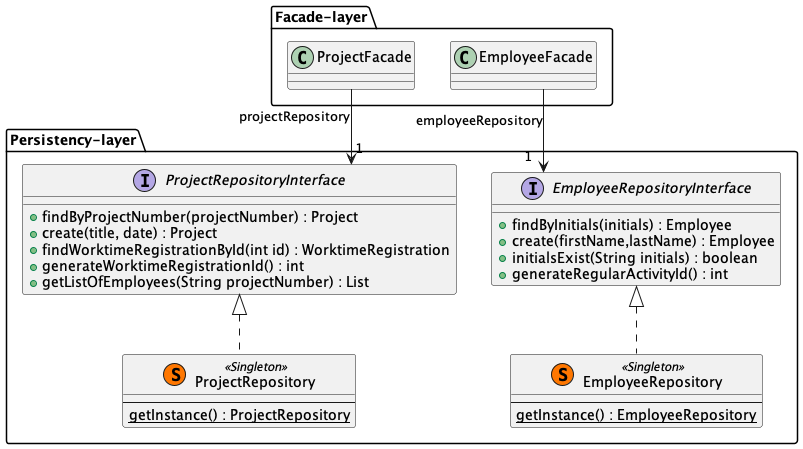
\includegraphics[width = 12cm, keepaspectratio]{TaskFusion/out/assets/diagrams/class_persistency_to_facade_improved/persistency_to_facade_example.png}
    \label{fig:class_facade_persistency_improved}
\end{figure}

\subsection{Dependency inversion principle} \label{sec:solid_d}
Med et fortsat fokus på facade-laget og figur \ref{fig:class_facade_full}, implementere \texttt{EmployeeFacade} og \texttt{ProjectFacade} flere interfaces hver. På den måde kan mindre og fokuserede interfaces gøre det nemmere for facade klasserne at implementere de metoder, de har behov for.
\\
Vi kan også fremhæve et andet eksempel på opfyldelse af \textit{Dependency inversion principle}. \texttt{ConvertibleToViewModelInterface} er et interface der adskiller konverteringslogikken fra domæneobjekterne, se klassediagram herunder i figur \ref{fig:class_convertible_example}. Klasser som \texttt{Project} og \texttt{Employee} implementerer dette interface og kan dermed konverteres til en \texttt{ViewModel} til brug i præsentationslaget. På denne måde har vi en simpel og fokuseret kontrakt for domæneobjekter, der kan udvide deres funktionalitet uden at ændre deres kerneadfærd. 

\begin{figure}[H]
    \centering
    \caption{Klassediagram af \textit{ConvertibleToViewModelInterface} implementeringer}
    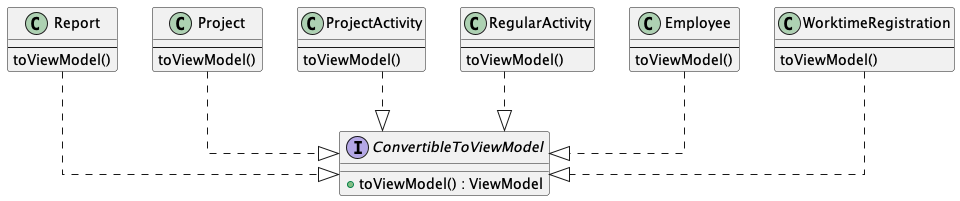
\includegraphics[width = \textwidth, keepaspectratio]{TaskFusion/out/assets/diagrams/class_convertibleToViewModel_example/ConvertibleToViewModel_diagram.png}
    \label{fig:class_convertible_example}
\end{figure}

